\documentclass[]{article}
\usepackage{lmodern}
\usepackage{amssymb,amsmath}
\usepackage{ifxetex,ifluatex}
\usepackage{fixltx2e} % provides \textsubscript
\ifnum 0\ifxetex 1\fi\ifluatex 1\fi=0 % if pdftex
  \usepackage[T1]{fontenc}
  \usepackage[utf8]{inputenc}
\else % if luatex or xelatex
  \ifxetex
    \usepackage{mathspec}
  \else
    \usepackage{fontspec}
  \fi
  \defaultfontfeatures{Ligatures=TeX,Scale=MatchLowercase}
\fi
% use upquote if available, for straight quotes in verbatim environments
\IfFileExists{upquote.sty}{\usepackage{upquote}}{}
% use microtype if available
\IfFileExists{microtype.sty}{%
\usepackage{microtype}
\UseMicrotypeSet[protrusion]{basicmath} % disable protrusion for tt fonts
}{}
\usepackage[margin=1in]{geometry}
\usepackage{hyperref}
\hypersetup{unicode=true,
            pdftitle={Linear Regression - Airbnb data},
            pdfborder={0 0 0},
            breaklinks=true}
\urlstyle{same}  % don't use monospace font for urls
\usepackage{color}
\usepackage{fancyvrb}
\newcommand{\VerbBar}{|}
\newcommand{\VERB}{\Verb[commandchars=\\\{\}]}
\DefineVerbatimEnvironment{Highlighting}{Verbatim}{commandchars=\\\{\}}
% Add ',fontsize=\small' for more characters per line
\usepackage{framed}
\definecolor{shadecolor}{RGB}{248,248,248}
\newenvironment{Shaded}{\begin{snugshade}}{\end{snugshade}}
\newcommand{\AlertTok}[1]{\textcolor[rgb]{0.94,0.16,0.16}{#1}}
\newcommand{\AnnotationTok}[1]{\textcolor[rgb]{0.56,0.35,0.01}{\textbf{\textit{#1}}}}
\newcommand{\AttributeTok}[1]{\textcolor[rgb]{0.77,0.63,0.00}{#1}}
\newcommand{\BaseNTok}[1]{\textcolor[rgb]{0.00,0.00,0.81}{#1}}
\newcommand{\BuiltInTok}[1]{#1}
\newcommand{\CharTok}[1]{\textcolor[rgb]{0.31,0.60,0.02}{#1}}
\newcommand{\CommentTok}[1]{\textcolor[rgb]{0.56,0.35,0.01}{\textit{#1}}}
\newcommand{\CommentVarTok}[1]{\textcolor[rgb]{0.56,0.35,0.01}{\textbf{\textit{#1}}}}
\newcommand{\ConstantTok}[1]{\textcolor[rgb]{0.00,0.00,0.00}{#1}}
\newcommand{\ControlFlowTok}[1]{\textcolor[rgb]{0.13,0.29,0.53}{\textbf{#1}}}
\newcommand{\DataTypeTok}[1]{\textcolor[rgb]{0.13,0.29,0.53}{#1}}
\newcommand{\DecValTok}[1]{\textcolor[rgb]{0.00,0.00,0.81}{#1}}
\newcommand{\DocumentationTok}[1]{\textcolor[rgb]{0.56,0.35,0.01}{\textbf{\textit{#1}}}}
\newcommand{\ErrorTok}[1]{\textcolor[rgb]{0.64,0.00,0.00}{\textbf{#1}}}
\newcommand{\ExtensionTok}[1]{#1}
\newcommand{\FloatTok}[1]{\textcolor[rgb]{0.00,0.00,0.81}{#1}}
\newcommand{\FunctionTok}[1]{\textcolor[rgb]{0.00,0.00,0.00}{#1}}
\newcommand{\ImportTok}[1]{#1}
\newcommand{\InformationTok}[1]{\textcolor[rgb]{0.56,0.35,0.01}{\textbf{\textit{#1}}}}
\newcommand{\KeywordTok}[1]{\textcolor[rgb]{0.13,0.29,0.53}{\textbf{#1}}}
\newcommand{\NormalTok}[1]{#1}
\newcommand{\OperatorTok}[1]{\textcolor[rgb]{0.81,0.36,0.00}{\textbf{#1}}}
\newcommand{\OtherTok}[1]{\textcolor[rgb]{0.56,0.35,0.01}{#1}}
\newcommand{\PreprocessorTok}[1]{\textcolor[rgb]{0.56,0.35,0.01}{\textit{#1}}}
\newcommand{\RegionMarkerTok}[1]{#1}
\newcommand{\SpecialCharTok}[1]{\textcolor[rgb]{0.00,0.00,0.00}{#1}}
\newcommand{\SpecialStringTok}[1]{\textcolor[rgb]{0.31,0.60,0.02}{#1}}
\newcommand{\StringTok}[1]{\textcolor[rgb]{0.31,0.60,0.02}{#1}}
\newcommand{\VariableTok}[1]{\textcolor[rgb]{0.00,0.00,0.00}{#1}}
\newcommand{\VerbatimStringTok}[1]{\textcolor[rgb]{0.31,0.60,0.02}{#1}}
\newcommand{\WarningTok}[1]{\textcolor[rgb]{0.56,0.35,0.01}{\textbf{\textit{#1}}}}
\usepackage{longtable,booktabs}
\usepackage{graphicx,grffile}
\makeatletter
\def\maxwidth{\ifdim\Gin@nat@width>\linewidth\linewidth\else\Gin@nat@width\fi}
\def\maxheight{\ifdim\Gin@nat@height>\textheight\textheight\else\Gin@nat@height\fi}
\makeatother
% Scale images if necessary, so that they will not overflow the page
% margins by default, and it is still possible to overwrite the defaults
% using explicit options in \includegraphics[width, height, ...]{}
\setkeys{Gin}{width=\maxwidth,height=\maxheight,keepaspectratio}
\IfFileExists{parskip.sty}{%
\usepackage{parskip}
}{% else
\setlength{\parindent}{0pt}
\setlength{\parskip}{6pt plus 2pt minus 1pt}
}
\setlength{\emergencystretch}{3em}  % prevent overfull lines
\providecommand{\tightlist}{%
  \setlength{\itemsep}{0pt}\setlength{\parskip}{0pt}}
\setcounter{secnumdepth}{0}
% Redefines (sub)paragraphs to behave more like sections
\ifx\paragraph\undefined\else
\let\oldparagraph\paragraph
\renewcommand{\paragraph}[1]{\oldparagraph{#1}\mbox{}}
\fi
\ifx\subparagraph\undefined\else
\let\oldsubparagraph\subparagraph
\renewcommand{\subparagraph}[1]{\oldsubparagraph{#1}\mbox{}}
\fi

%%% Use protect on footnotes to avoid problems with footnotes in titles
\let\rmarkdownfootnote\footnote%
\def\footnote{\protect\rmarkdownfootnote}

%%% Change title format to be more compact
\usepackage{titling}

% Create subtitle command for use in maketitle
\providecommand{\subtitle}[1]{
  \posttitle{
    \begin{center}\large#1\end{center}
    }
}

\setlength{\droptitle}{-2em}

  \title{Linear Regression - Airbnb data}
    \pretitle{\vspace{\droptitle}\centering\huge}
  \posttitle{\par}
    \author{}
    \preauthor{}\postauthor{}
    \date{}
    \predate{}\postdate{}
  

\begin{document}
\maketitle

\begin{center}\rule{0.5\linewidth}{\linethickness}\end{center}

Load up Libraries

\begin{Shaded}
\begin{Highlighting}[]
\KeywordTok{library}\NormalTok{(dplyr)}
\KeywordTok{library}\NormalTok{(ggplot2)}
\KeywordTok{library}\NormalTok{(GGally)}
\end{Highlighting}
\end{Shaded}

\hypertarget{airbnb-data}{%
\subsection{Airbnb Data}\label{airbnb-data}}

\begin{Shaded}
\begin{Highlighting}[]
\NormalTok{airbnb_df =}\StringTok{ }\KeywordTok{read.csv}\NormalTok{(}\KeywordTok{paste}\NormalTok{(path,}\StringTok{"airbnb_data.csv"}\NormalTok{,}\DataTypeTok{sep=}\StringTok{""}\NormalTok{))}
\NormalTok{knitr}\OperatorTok{::}\KeywordTok{kable}\NormalTok{(}\KeywordTok{head}\NormalTok{(airbnb_df, }\DecValTok{4}\NormalTok{), }\StringTok{"pandoc"}\NormalTok{)}
\end{Highlighting}
\end{Shaded}

\begin{longtable}[]{@{}rrrllrrrrr@{}}
\toprule
room\_id & survey\_id & host\_id & room\_type & city & reviews &
overall\_satisfaction & accommodates & bedrooms & price\tabularnewline
\midrule
\endhead
15771735 & 1498 & 101992409 & Shared room & Asheville & 0 & 0.0 & 4 & 1
& 67\tabularnewline
18284194 & 1498 & 126414164 & Shared room & Asheville & 32 & 5.0 & 4 & 1
& 76\tabularnewline
18091012 & 1498 & 122380971 & Shared room & Asheville & 4 & 4.5 & 2 & 1
& 45\tabularnewline
12286328 & 1498 & 746673 & Shared room & Asheville & 24 & 4.5 & 6 & 1 &
26\tabularnewline
\bottomrule
\end{longtable}

\hypertarget{lets-fit-a-multiple-linear-regression-model-using-price-as-the-response-variable-and-all-others-as-predictor-variables-note-remove-id-columns.-we-will-check-which-variables-are-statistically-significant-in-determining-the-price.}{%
\paragraph{Let's fit a multiple linear regression model using price as
the response variable and all others as predictor variables (Note:
remove `id' columns). We will check which variables are statistically
significant in determining the
price.}\label{lets-fit-a-multiple-linear-regression-model-using-price-as-the-response-variable-and-all-others-as-predictor-variables-note-remove-id-columns.-we-will-check-which-variables-are-statistically-significant-in-determining-the-price.}}

\begin{Shaded}
\begin{Highlighting}[]
\CommentTok{#Remove all 'id' columns first}
\NormalTok{airbnb_df_no_ID =}\StringTok{ }\KeywordTok{select}\NormalTok{(airbnb_df, }\OperatorTok{-}\KeywordTok{contains}\NormalTok{(}\StringTok{"id"}\NormalTok{))}
\NormalTok{knitr}\OperatorTok{::}\KeywordTok{kable}\NormalTok{(}\KeywordTok{head}\NormalTok{(airbnb_df_no_ID, }\DecValTok{4}\NormalTok{), }\StringTok{"pandoc"}\NormalTok{)}
\end{Highlighting}
\end{Shaded}

\begin{longtable}[]{@{}llrrrrr@{}}
\toprule
room\_type & city & reviews & overall\_satisfaction & accommodates &
bedrooms & price\tabularnewline
\midrule
\endhead
Shared room & Asheville & 0 & 0.0 & 4 & 1 & 67\tabularnewline
Shared room & Asheville & 32 & 5.0 & 4 & 1 & 76\tabularnewline
Shared room & Asheville & 4 & 4.5 & 2 & 1 & 45\tabularnewline
Shared room & Asheville & 24 & 4.5 & 6 & 1 & 26\tabularnewline
\bottomrule
\end{longtable}

\begin{Shaded}
\begin{Highlighting}[]
\CommentTok{#Create Multiple Linear Regression Model}
\CommentTok{#Not mentioned in the question, but apparently this df only contains one city "Asheville"}
\CommentTok{#We will not include that in the model as it is not useful}
\NormalTok{air_MLM =}\StringTok{ }\KeywordTok{lm}\NormalTok{(price }\OperatorTok{~}\StringTok{ }\NormalTok{room_type }\OperatorTok{+}\StringTok{ }\NormalTok{reviews }\OperatorTok{+}\StringTok{ }\NormalTok{overall_satisfaction }\OperatorTok{+}\StringTok{ }\NormalTok{accommodates }\OperatorTok{+}\StringTok{ }\NormalTok{bedrooms, }\DataTypeTok{data=}\NormalTok{airbnb_df_no_ID)}

\CommentTok{#Display model output}
\KeywordTok{summary}\NormalTok{(air_MLM)}
\end{Highlighting}
\end{Shaded}

\begin{verbatim}
## 
## Call:
## lm(formula = price ~ room_type + reviews + overall_satisfaction + 
##     accommodates + bedrooms, data = airbnb_df_no_ID)
## 
## Residuals:
##    Min     1Q Median     3Q    Max 
## -367.8  -49.2    3.2   38.6 4032.7 
## 
## Coefficients:
##                        Estimate Std. Error t value Pr(>|t|)    
## (Intercept)           -23.36172   21.88618  -1.067  0.28609    
## room_typePrivate room  -0.93115   13.21827  -0.070  0.94386    
## room_typeShared room  -76.66780   59.90939  -1.280  0.20099    
## reviews                 0.01090    0.09982   0.109  0.91310    
## overall_satisfaction  -10.48160    3.47320  -3.018  0.00262 ** 
## accommodates           23.00721    5.23952   4.391 1.27e-05 ***
## bedrooms               85.64533   11.45983   7.474 1.95e-13 ***
## ---
## Signif. codes:  0 '***' 0.001 '**' 0.01 '*' 0.05 '.' 0.1 ' ' 1
## 
## Residual standard error: 167.1 on 847 degrees of freedom
## Multiple R-squared:  0.3228, Adjusted R-squared:  0.318 
## F-statistic:  67.3 on 6 and 847 DF,  p-value: < 2.2e-16
\end{verbatim}

As we can see from the above summary output from the model, the
variables that are statistically significant in determining price are:
\textbf{``overall\_satisfaction''}, \textbf{``accommodates''} and
\textbf{``bedrooms''}. This is assuming an alpha value of .05.

\hypertarget{how-would-we-interpret-coefficients-for-predictors}{%
\subsubsection{How would we interpret coefficients for
predictors?}\label{how-would-we-interpret-coefficients-for-predictors}}

\begin{itemize}
\tightlist
\item
  Ex.1) A shared room is associated with a decrease of \$76.67 in price
  on average holding all else constant.
\item
  Ex.2) A one unit increase in bedrooms (so each additional bedroom) is
  associated with an increase of \$85.65 in price on average holding all
  else constant.
\end{itemize}

\hypertarget{lets-take-an-example-and-predict-the-price-using-the-above-multiple-linear-model.-how-about-a-listing-with-1-bedroom-that-can-accomodate-2-people-with-total-of-70-reviews-with-mean-rating-of-4-that-is-a-private-room.-what-does-our-model-estimate-its-rental-price-should-be}{%
\paragraph{Let's take an example and predict the price using the above
multiple linear model. How about a listing with 1 bedroom that can
accomodate 2 people, with total of 70 reviews with mean rating of 4 that
is a private room. What does our model estimate its rental price should
be?}\label{lets-take-an-example-and-predict-the-price-using-the-above-multiple-linear-model.-how-about-a-listing-with-1-bedroom-that-can-accomodate-2-people-with-total-of-70-reviews-with-mean-rating-of-4-that-is-a-private-room.-what-does-our-model-estimate-its-rental-price-should-be}}

\begin{Shaded}
\begin{Highlighting}[]
\NormalTok{pred_data =}\StringTok{ }\KeywordTok{data.frame}\NormalTok{(}\DataTypeTok{bedrooms=}\DecValTok{1}\NormalTok{, }\DataTypeTok{accommodates=}\DecValTok{2}\NormalTok{, }\DataTypeTok{reviews=}\DecValTok{70}\NormalTok{, }\DataTypeTok{overall_satisfaction=}\DecValTok{4}\NormalTok{, }\DataTypeTok{room_type=}\StringTok{'Private room'}\NormalTok{)}
\CommentTok{#Prediction using Prediction interval}
\NormalTok{air_MLM_pred =}\StringTok{ }\KeywordTok{predict}\NormalTok{(air_MLM, pred_data, }\DataTypeTok{interval =} \StringTok{"predict"}\NormalTok{)}
\NormalTok{air_MLM_pred}
\end{Highlighting}
\end{Shaded}

\begin{verbatim}
##        fit       lwr      upr
## 1 66.20316 -262.3605 394.7669
\end{verbatim}

As we can see from the output of the prediction above, with the
following factor values: bedrooms = 1, accommodates = 2, reviews = 70,
overall\_satisfaction = 4, and room\_type = `Private room' the predicted
price is \$66.

As an aside, when doing predictions, I will include both prediction and
confidence intervals so we can compere the lower and upper bounds.

\begin{quote}
For additional edification on which you should use: According to ISLR we
should use a prediction interval if we wish to predict an individual
response and use a confidence interval if we wish to predict the average
response. Also, this
\href{http://www.sthda.com/english/articles/40-regression-analysis/166-predict-in-r-model-predictions-and-confidence-intervals/}{article}
sums it up nicely. From the article, ``A prediction interval reflects
the uncertainty around a single value, while a confidence interval
reflects the uncertainty around the mean prediction values. Thus, a
prediction interval will be generally much wider than a confidence
interval for the same value.''
\end{quote}

Checkout this
\href{https://www.youtube.com/watch?feature=player_embedded\&v=o0UESA3UZss}{video}
for more context on confidence interval vs.~prediction interval:
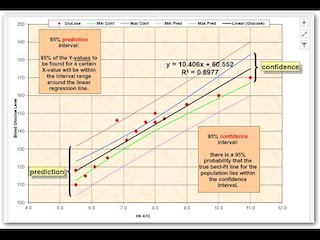
\includegraphics{/Users/young.cho/Documents/portfolio/portfolio/media/ci_vs_pi.jpg}

\hypertarget{next-lets-identify-outliers-using-cooks-distance-approach.}{%
\paragraph{Next let's identify outliers using Cook's distance
approach.}\label{next-lets-identify-outliers-using-cooks-distance-approach.}}

Identify outliers using Cook's distance approach. Remove points having
Cook's distance \textgreater{} 1. Rerun the model after the removal of
these points and print the summary.

\begin{Shaded}
\begin{Highlighting}[]
\CommentTok{#Find leverage points using the Residuals vs Leverage plot}
\CommentTok{#Cook's distance > 1 }
\KeywordTok{plot}\NormalTok{(air_MLM, }\DataTypeTok{which =} \DecValTok{5}\NormalTok{)}
\end{Highlighting}
\end{Shaded}

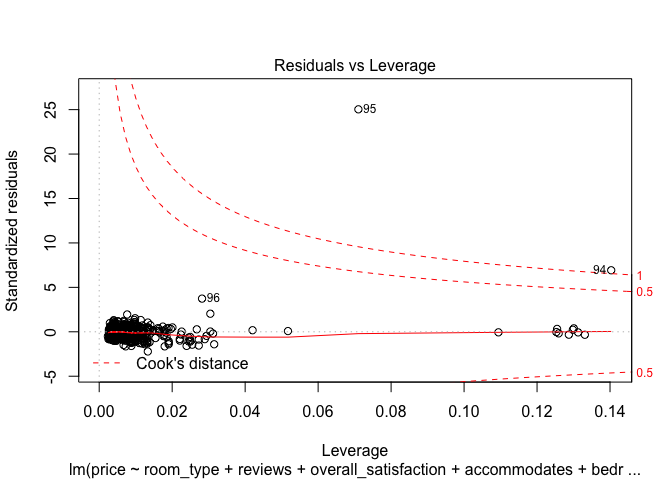
\includegraphics{linear_regression_01_files/figure-latex/unnamed-chunk-7-1.pdf}

\begin{Shaded}
\begin{Highlighting}[]
\CommentTok{#Remove identified leverage points}
\NormalTok{airbnb_df_no_ID_clean =}\StringTok{ }\NormalTok{airbnb_df_no_ID[}\OperatorTok{-}\KeywordTok{c}\NormalTok{(}\DecValTok{94}\NormalTok{, }\DecValTok{95}\NormalTok{),]}

\CommentTok{#Rerun the model after removing points where Cook's distance is > 1}
\NormalTok{air_MLM_clean =}\StringTok{ }\KeywordTok{lm}\NormalTok{(price }\OperatorTok{~}\StringTok{ }\NormalTok{room_type }\OperatorTok{+}\StringTok{ }\NormalTok{reviews }\OperatorTok{+}\StringTok{ }\NormalTok{overall_satisfaction }\OperatorTok{+}\StringTok{ }\NormalTok{accommodates }\OperatorTok{+}\StringTok{ }\NormalTok{bedrooms, }\DataTypeTok{data=}\NormalTok{airbnb_df_no_ID_clean)}
\KeywordTok{summary}\NormalTok{(air_MLM_clean)}
\end{Highlighting}
\end{Shaded}

\begin{verbatim}
## 
## Call:
## lm(formula = price ~ room_type + reviews + overall_satisfaction + 
##     accommodates + bedrooms, data = airbnb_df_no_ID_clean)
## 
## Residuals:
##     Min      1Q  Median      3Q     Max 
## -190.95  -32.43   -7.09   20.35  876.26 
## 
## Coefficients:
##                        Estimate Std. Error t value Pr(>|t|)    
## (Intercept)            75.01310    9.09152   8.251 6.01e-16 ***
## room_typePrivate room -32.28201    5.38034  -6.000 2.92e-09 ***
## room_typeShared room  -91.69951   24.28958  -3.775 0.000171 ***
## reviews                -0.05915    0.04047  -1.462 0.144202    
## overall_satisfaction   -6.78957    1.41118  -4.811 1.78e-06 ***
## accommodates           11.90698    2.14267   5.557 3.68e-08 ***
## bedrooms               35.93177    4.87968   7.364 4.25e-13 ***
## ---
## Signif. codes:  0 '***' 0.001 '**' 0.01 '*' 0.05 '.' 0.1 ' ' 1
## 
## Residual standard error: 67.73 on 845 degrees of freedom
## Multiple R-squared:  0.4249, Adjusted R-squared:  0.4208 
## F-statistic:   104 on 6 and 845 DF,  p-value: < 2.2e-16
\end{verbatim}

Isn't this facinating? The summary output seems to make way more logical
sense now. After removing records 94 and 95, where Cook's distance
\textgreater{} 1, the only X variable that doesn't look significant is
now reviews. Assuming an alpha of .05, all other predictor variables
look significant to the model. We can also see from the newly plotted
Residuals vs Leverage plot that no values exceed Cook's distance
\textgreater{} 1.

And next let's run a new prediction model using the cleaned data set.

\begin{Shaded}
\begin{Highlighting}[]
\CommentTok{#Predicting using confidence interval}
\NormalTok{air_MLM_pred_clean =}\StringTok{ }\KeywordTok{predict}\NormalTok{(air_MLM_clean, pred_data, }\DataTypeTok{interval =} \StringTok{"confidence"}\NormalTok{)}
\NormalTok{air_MLM_pred_clean}
\end{Highlighting}
\end{Shaded}

\begin{verbatim}
##        fit      lwr      upr
## 1 71.17796 63.65645 78.69946
\end{verbatim}

\begin{Shaded}
\begin{Highlighting}[]
\CommentTok{#predicting using Prediction interval}
\NormalTok{air_MLM_pred_clean =}\StringTok{ }\KeywordTok{predict}\NormalTok{(air_MLM_clean, pred_data, }\DataTypeTok{interval =} \StringTok{"prediction"}\NormalTok{)}
\NormalTok{air_MLM_pred_clean}
\end{Highlighting}
\end{Shaded}

\begin{verbatim}
##        fit       lwr      upr
## 1 71.17796 -61.98274 204.3387
\end{verbatim}

Compared to our first prediction, the new prediction has much narrower
lower and upper bands with a predicted value of \$71.


\end{document}
